\documentclass[tikz,border=3pt]{standalone}
\usepackage[utf8]{inputenc}
\usepackage[T1]{fontenc}
\usepackage{lmodern}
\renewcommand{\familydefault}{\sfdefault}
\usepackage{sansmath}\sansmath
\usepackage{chemfig}
\usepackage{pgfplots}\pgfplotsset{compat=1.18,/pgf/number format/use comma,/pgf/number format/1000 sep={.}}
\usetikzlibrary{arrows.meta,calc,positioning,decorations.pathmorphing,patterns}
% paleta del sitio
\definecolor{nar}{HTML}{E8680C}\definecolor{narc}{HTML}{FFB35C}\definecolor{hielo}{HTML}{FFF3E8}
\definecolor{tinta}{HTML}{1D1D1F}\definecolor{gris}{HTML}{6E6E73}\definecolor{lila}{HTML}{7C5CF0}
\definecolor{azul}{HTML}{2F6FD6}\definecolor{menta}{HTML}{17A673}\definecolor{coral}{HTML}{E8342A}
\begin{document}
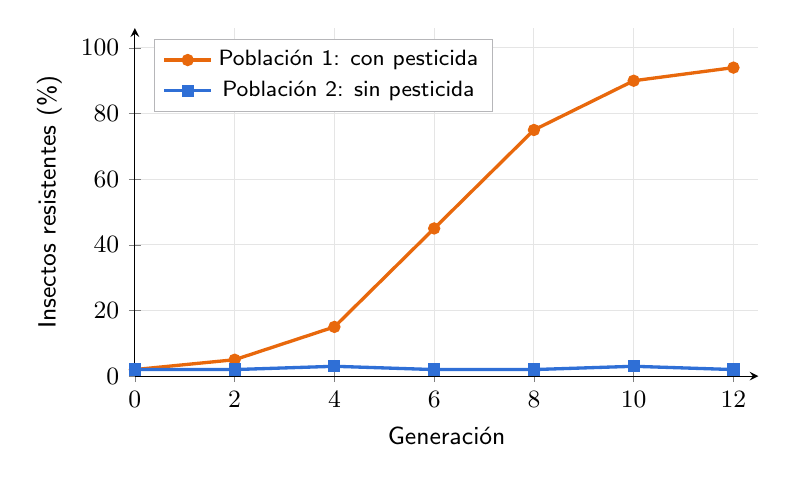
\begin{tikzpicture}[font=\small]
\begin{axis}[width=9.5cm,height=6cm,axis lines=left,grid=major,grid style={gray!20},
  xmin=0,xmax=12.5,ymin=0,ymax=106,xtick={0,2,...,12},ytick={0,20,...,100},
  xlabel={Generación},ylabel={Insectos resistentes (\%)},
  legend style={at={(0.03,0.97)},anchor=north west,font=\footnotesize,draw=gris!50}]
\addplot[nar,very thick,mark=*,mark options={scale=0.8,fill=nar}] coordinates {(0,2)(2,5)(4,15)(6,45)(8,75)(10,90)(12,94)};
\addlegendentry{Población 1: con pesticida}
\addplot[azul,very thick,mark=square*,mark options={scale=0.8,fill=azul}] coordinates {(0,2)(2,2)(4,3)(6,2)(8,2)(10,3)(12,2)};
\addlegendentry{Población 2: sin pesticida}
\end{axis}
\end{tikzpicture}
\end{document}
